\documentclass[10pt,twocolumn,letterpaper]{article}

\usepackage{../cvpr}
\usepackage{times}
\usepackage{epsfig}
\usepackage{graphicx}
\usepackage{amsmath}
\usepackage{amssymb}

% Include other packages here, before hyperref.

% If you comment hyperref and then uncomment it, you should delete
% egpaper.aux before re-running latex.  (Or just hit 'q' on the first latex
% run, let it finish, and you should be clear).
\usepackage[pagebackref=true,breaklinks=true,letterpaper=true,colorlinks,bookmarks=false]{hyperref}

\cvprfinalcopy % *** Uncomment this line for the final submission

\def\cvprPaperID{****} % *** Enter the CVPR Paper ID here
\def\httilde{\mbox{\tt\raisebox{-.5ex}{\symbol{126}}}}

% Pages are numbered in submission mode, and unnumbered in camera-ready
\ifcvprfinal\pagestyle{empty}\fi

\begin{document}
	
	\title{Differentiable Particle Filters: End-to-End Learning with Algorithmic Priors}
	\author{Rico Jonschkowski \and Divyam Rastogi\and Oliver Brock}
	\date{May 2018}
	
	\maketitle

	\section{Motivation}
	The architecture proposed in this work is motivated by the benefits of:
	\begin{itemize}
		\item \textbf{End-to-end learning} over learn the components of an architecture separately since it provides more generality, and
		\item \textbf{Algorithmic Priors} in the context of end-to-end learning, since a naive application of the latter may lead to overfitting.
	\end{itemize}
	The authors cite here the success of \textbf{CNNs}, an algorithmic prior for end-to-end learning of architectures for image-based tasks like segmentation.
	
	\section{Problem Statement}
	
	The goal we are working towards is estimating the state $z_[1:T]$ in a State Space Model: 
	
	%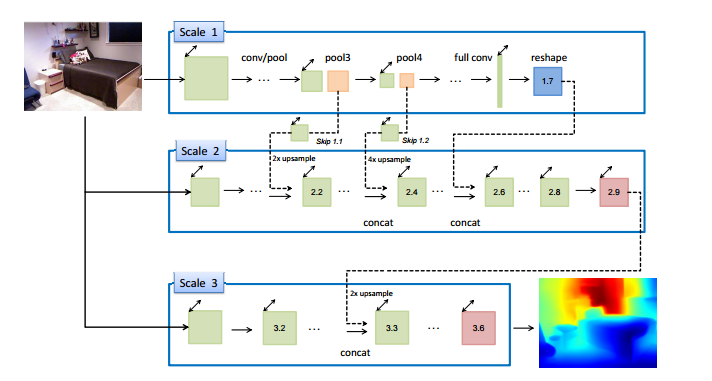
\includegraphics[width = 7.5cm, height = 4cm]{dlcv.png}
	\begin{figure}[htbp]
		\centering
		% The state vector is represented by a blue circle.
		% "minimum size" makes sure all circles have the same size
		% independently of their contents.
		\tikzstyle{state}=[circle,
		thick,
		minimum size=1.0cm,
		draw=black!80,
		fill=gray!20]
		
		% The measurement vector is represented by an orange circle.
		\tikzstyle{measurement}=[circle,
		thick,
		minimum size=1.0cm,
		draw=black!80,
		fill=purple!25]
		
		% The control input vector is represented by a purple circle.
		\tikzstyle{input}=[circle,
		thick,
		minimum size=1.0cm,
		draw=black!80,
		fill=white!20]
		
		\begin{tikzpicture}[>=latex,text height=1.5ex,text depth=0.25ex]
		% "text height" and "text depth" are required to vertically
		% align the labels with and without indices.
		
		% The various elements are conveniently placed using a matrix:
		\matrix[row sep=0.2cm,column sep=0.2cm] {
			% First line: States
			\node (z_k-2) 		 {$\cdots$};      	   &
			\node (z_k-1) [state]{$\mathbf{z}_{k-1}$}; &
			&
			\node (z_k)   [state]{$\mathbf{z}_k$};     &
			&
			\node (z_k+1) [state]{$\mathbf{z}_{k+1}$}; &
			\\
			% Second line: inputs
			\node (u_k-1) [input] {$\mathbf{u}_{k-1}$}; &
			&
			\node (u_k)   [input] {$\mathbf{u}_k$};     &
			&
			\node (u_k+1) [input] {$\mathbf{u}_{k+1}$}; &
			&
			\\
			% Third line: measurements
			&
			\node (x_k-1) [measurement] {$\mathbf{x}_{k-1}$};       &
			&
			\node (x_k)   [measurement] {$\mathbf{x}_{k}$};       &
			&
			\node (x_k+1) [measurement] {$\mathbf{x}_{k+1}$};       &
			\\
		};
		
		% The diagram elements are now connected through arrows:
		\path[->]
		(u_k-1) edge[thick] (z_k-1)
		(u_k) 	edge[thick] (z_k)	
		(u_k+1) edge[thick] (z_k+1)		
		(z_k-1) edge[thick] (x_k-1)	
		(z_k) 	edge[thick] (x_k)	
		(z_k+1) edge[thick] (x_k+1)		
		(z_k-2) edge[thick] (z_k-1)
		(z_k-1)	edge[thick] (z_k)
		(z_k)	edge[thick] (z_k+1)	
		;
		
		% Now that the diagram has been drawn, background rectangles
		% can be fitted to its elements. This requires the TikZ
		% libraries "fit" and "background".
		% Control input and measurement are labeled. These labels have
		% not been translated to English as "Measurement" instead of
		% "Messung" would not look good due to it being too long a word.
		
		% \begin{pgfonlayer}{background}
		% \node [background,
		% fit=(u_k-1) (u_k+1),
		% label=left:Entrance:] {};
		% \node [background,
		% fit=(w_k-1) (v_k-1) (A_k+1)] {};
		% \node [background,
		% fit=(z_k-1) (z_k+1),
		% label=left:Measure:] {};
		% \end{pgfonlayer}
		\end{tikzpicture}
		
		\caption{State Space Model}
		\label{fig:SSM}
	\end{figure}
	
	given just the observations $x_{1:T}$ and actions $u_{1:T}$. Essentially, what we want is a probability distribution over states at every time step $t$ (to account for uncertainty). We often encode this in the form of filtering distributions or beliefs:
	\begin{equation}
	bel{z_t} = p(z_t|x_{1:t}, u_{1:t})
	\end{equation}
	
	\section{Theoretical Background for solution}
	
	\subsection{Bayes Filter: Algorithmic Priors for State Estimation in Robotics}
	
	The authors argue that the \textbf{Bayes Filter} is a suitable algorithmic prior for learning a model that can estimate the system state (for systems that follow a generative model like the one in Figure \ref{fig:SSM}).
	
	The Bayes Filter calculates the belief over states at each point of time using two steps iteratively over the whole sequence:
	
	\begin{itemize}
		\item \textbf{Prediction:} This step predicts a distribution over the next state $z_{t}$ given the belief over the current state $z_{t-1}$. This is essentially done by calculating an expectation of the generative transition step $p(z_t|z_{t-1}, u_{t-1})$ w.r.t the belief over the current state:
		\begin{equation}
		bel(z_t) = \int{p(z_t|z_{t-1}, u_{t-1})}\overline{bel}(z_{t-1}) dz_{t-1}
		\end{equation}
		\item \textbf{Measurement:} This step updates the predicted belief $bel(z_t)$ to $\overline{bel}(z_{t})$ by incorporating the measurement $x_t$:
		\begin{equation}
		\overline{bel}(z_t) = \eta p(x_t|z_t)bel(z_t)
		\end{equation}
		where $\eta$ is the normalization constant ($p(x_t)$?)
	\end{itemize}
	
	Essentially,
	\begin{equation}
	bel(z_t) = p(z_t|x_{1:t-1}) \text{, and} 
	\end{equation}
	\begin{equation}
	\overline{bel}(z_t) = p(z_t|x_{1:t})
	\end{equation}
	
	\subsection{Particle Filter}
	Particle Filters are a class of Bayes Filters that \emph{approximate} the belief over states with several particles or samples ${z^{[1]}_t, z^{[2]}_t, ... z^{[N]}_t}$ that associated with corresponding weights ${w^{[1]}_t, w^{[2]}_t, ... w^{[N]}_t}$. The Bayes update steps in this context are:
	
	\begin{itemize}
		\item \textbf{Prediction} Sample N particles using a proposal distribution $q(z_t)$ (usually taken to be the generative transition distribution - $p(z_t|z_{t-1})$):
		\begin{equation}
		{z^{[1]}_t, z^{[2]}_t, ... z^{[N]}_t} \sim q(z_t)
		\end{equation}
		
		\item \textbf{Measurement} Calculate the un-normalized weights $\overline{w}$ for each of the particles using the emmision ($p(x_t|z_t)$), transition and the proposal distributions:
		\begin{equation}
		\overline{w}^{[i]}_t = \frac{p(x_t|z_t)p(z_t|z_{t-1})}{q(z_t)}
		\end{equation}
		Re-sample the N particles from a categorical distribution with parameters ${w^{[1]}_t, w^{[2]}_t, ... w^{[N]}_t}$, the normalized weights.  
		
	\end{itemize}
	
	\section{Method - DPF}
	In line with their motivation for end-to-end learning, the authors propose Differentiable Particle Filters, in which one learns the parameters ($\theta$) of the functions for each of the components necessary for a particle filter:
	\begin{itemize}
		\item \textbf{Action Sampler $f$} creates a noisy action to inject uncertainty into the transition model:		
			\begin{equation} \label{eq:dpf_as}
			\hat{u_t} = u_t + f_{\theta}(u_t, \epsilon \sim \mathcal{N}(0,1))
			\end{equation}
		\item \textbf{Generative Transition Model $g$} predicts the next state given the current state and action:
			\begin{equation} \label{eq:dpf_gp}
			z_{t+1} = z_{t} + g_{\theta}(z_{t}, \hat{u_{t}})
			\end{equation}
		\item \textbf{Encoder $h$} encodes the current observation $x_t$ into a low dimensional encoding:
			\begin{equation}
			e_t = h(x_t)
			\end{equation}
		\item \textbf{Proposer $k$} predicts the state given the encoding:
			\begin{equation}
			z^{[i]}_t = k(e_t, \delta^{[i]} \sim B))
			\end{equation}
			where $\delta^{[i]}$ is a dropout vector sampled from a Bernoulli distribution. This is to induce noise while getting the N particles.
		\item \textbf{Emmision $l$} weighs each particle based on the observation
			\begin{equation} \label{eq:dpf_wts}
			w^{[i]}_t = l(e_t, z_t)
			\end{equation}
	\end{itemize}
	
	The belief $bel(z_t)$ in this context is characterized by a set of particles and their corresponding weights, i.e:
	\begin{equation}
		bel(z_t) = \{ Z_t, W_t \} \text{, where } 
	\end{equation}
	\begin{equation*}
		Z_t = \{z^{[i]}_t\}_{i=1}^N \text{ and } W_t = \{w^{[i]}_t\}_{i=1}^N
	\end{equation*}
	
	The previous belief $bel(z_{t-1})$ is updated by the next set of particles which are either obtained by:
	\begin{itemize}
		\item \textbf{Prediction and Measurement update / Resampling}: \\
			State particles are obtained using the action sampler \ref{eq:dpf_as} and the generative prediction model \ref{eq:dpf_gp}, followed by a resampling according to weights that are obtained from \ref{eq:dpf_wts}
		\item \textbf{New particles from the proposer $k$}: \\
			New particles are obtained by directly using the observation $x_t$ at time step $t$ and their corresponding weights are calculated according to equation \ref{eq:dpf_wts}
	\end{itemize}
	
	\section{Training}
	
\end{document}